\documentclass{article}

\usepackage{graphicx}
\usepackage{tikz}
\usepackage{tikzsymbols}
\usetikzlibrary{calc,patterns,shapes.geometric}
\pagestyle{empty}
\usepackage[margin=0pt]{geometry}
\geometry{papersize={14in,12in}}

\def\centerarc[#1](#2)(#3:#4:#5){\draw[#1] ($(#2)+({#5*cos(#3)},{#5*sin(#3)})$) arc (#3:#4:#5);}

\begin{document}
	\begin{figure}
		\centering
		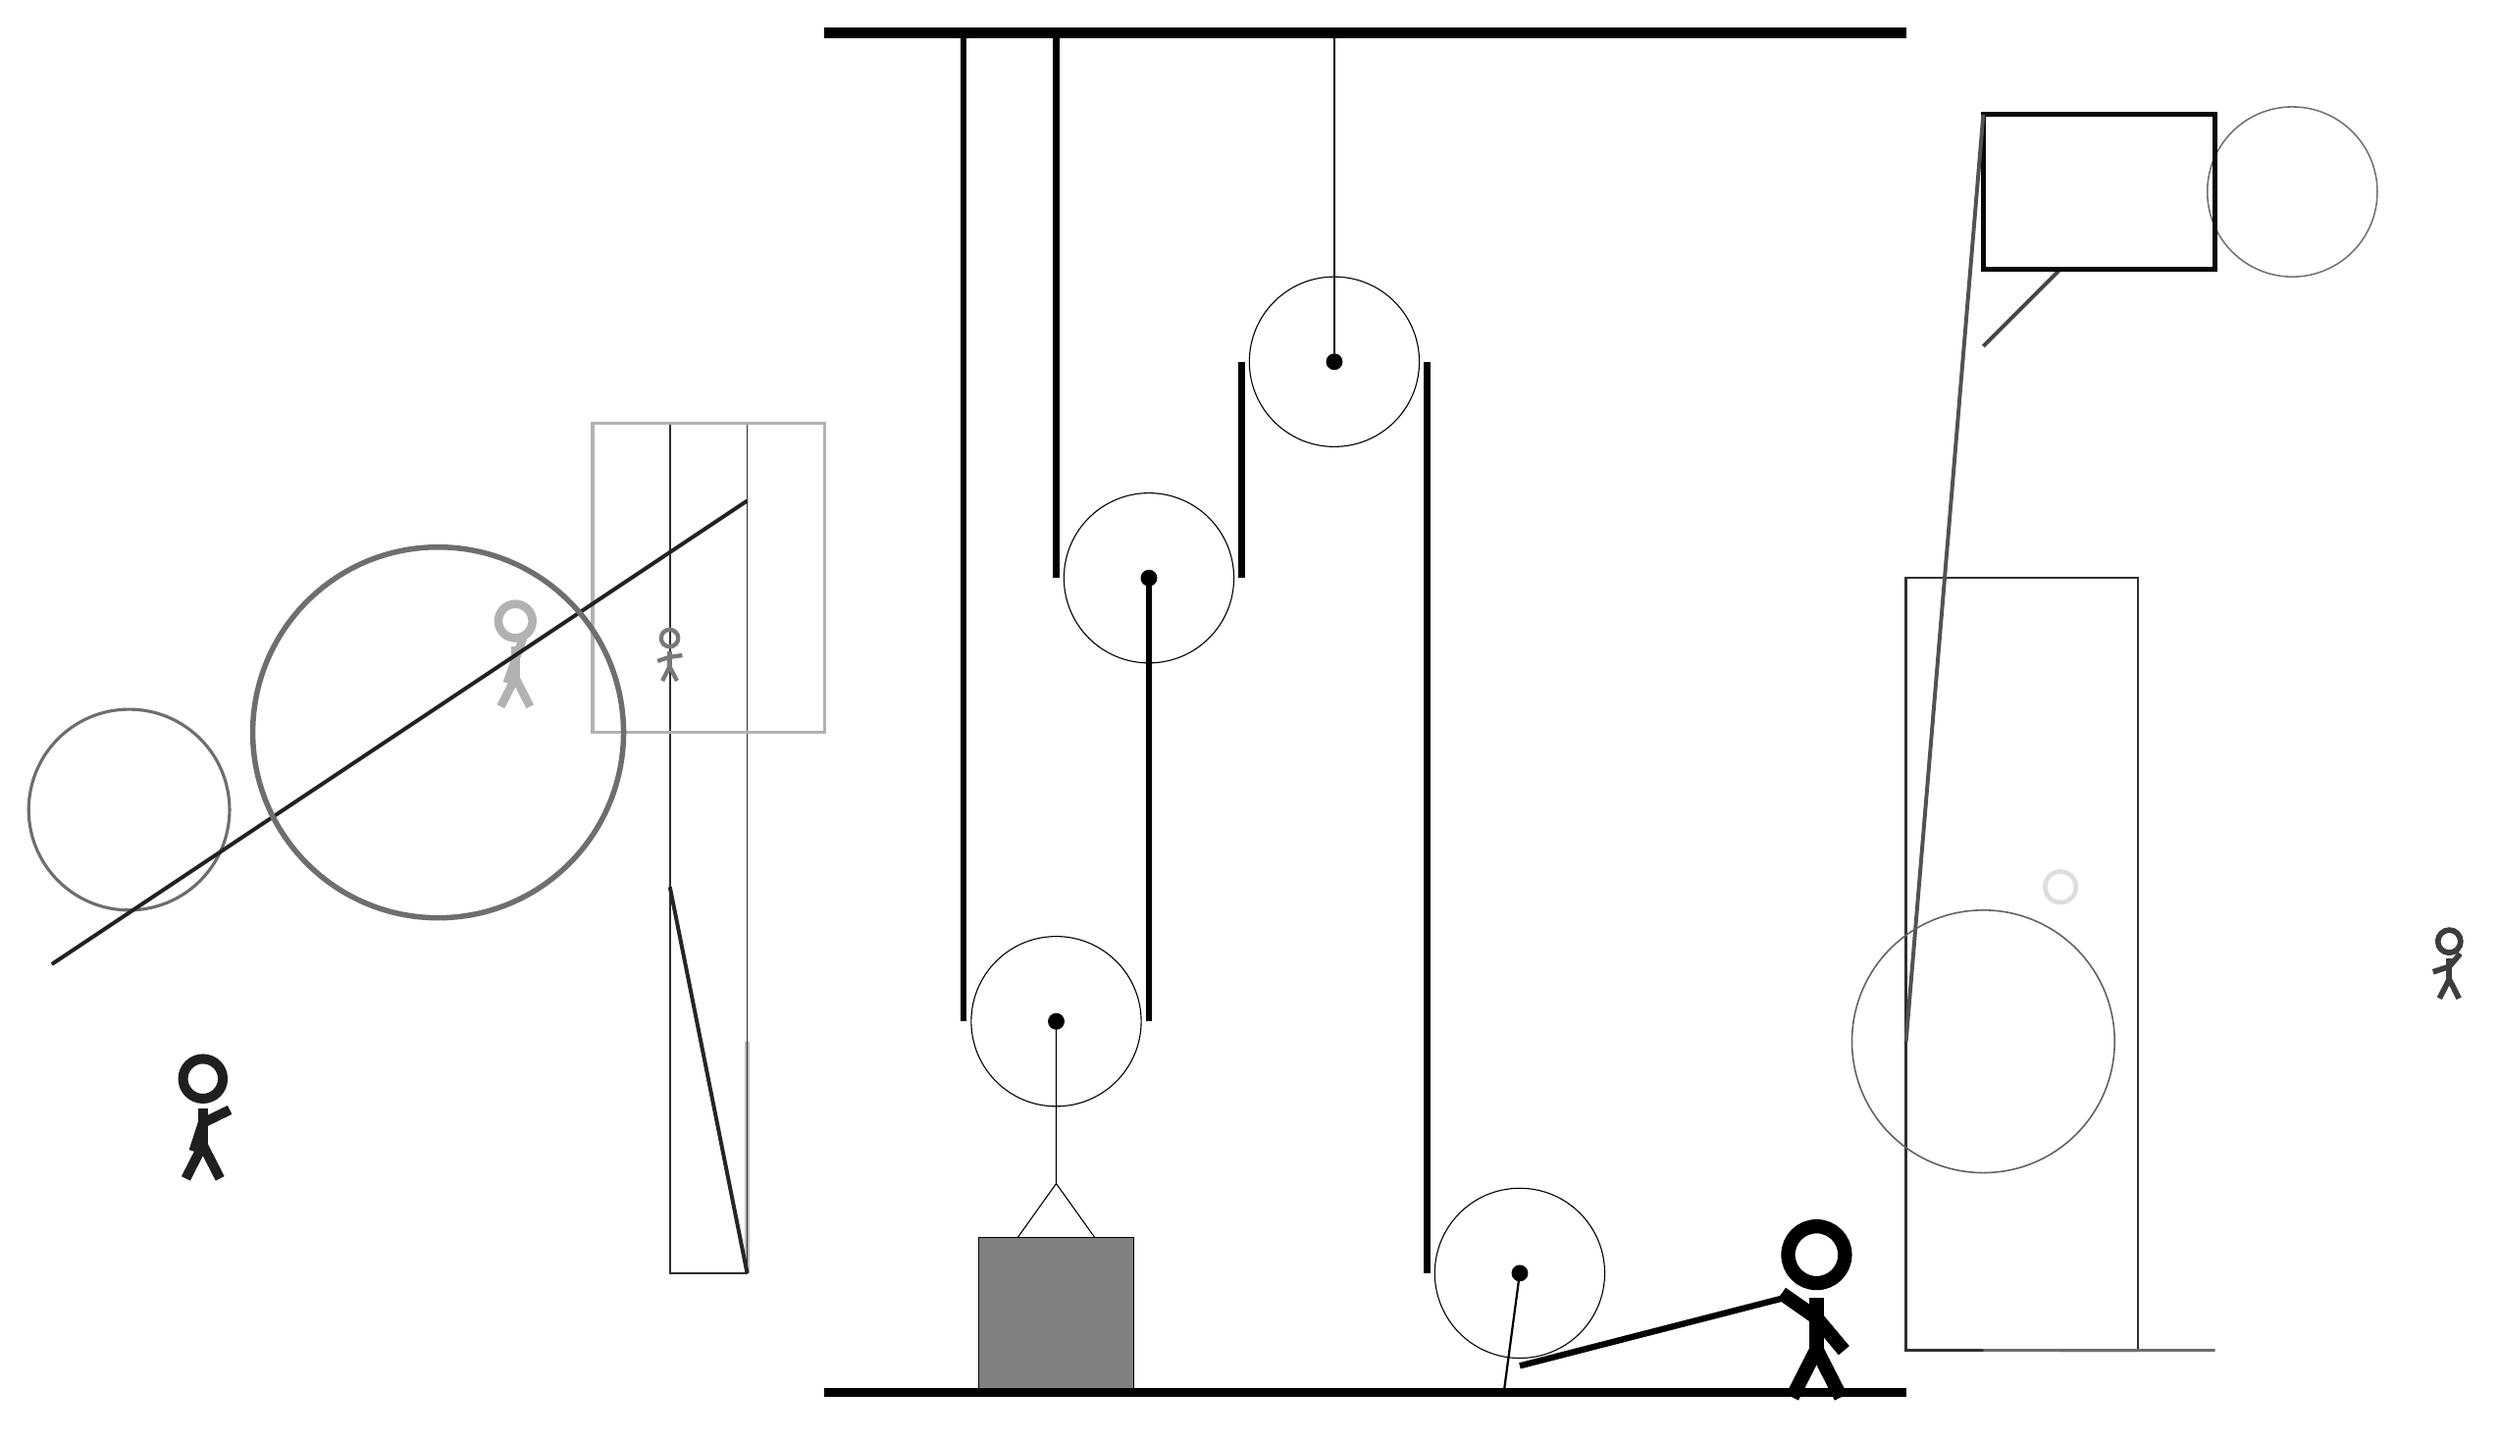
\begin{tikzpicture}
			%%%%% START %%%%%
			
			\draw[fill=black] (-2, 14) rectangle (12, 14.125);
			
			\draw (1, 1.26) circle (1.1);
			\draw[fill=black] (1, 1.26) circle (0.1);
			
			\draw (2.2, 7.0) circle (1.1);
			\draw[fill=black] (2.2, 7.0) circle (0.1);
			
			\draw[line width=0.5mm, color=black!73](13, 10) -- (14, 11);
			
			\node[line width=0.3mm, color=black!30] at (-6, 6) {\Strichmaxerl[6][71][70]};
			\node[line width=0.6mm, color=black!76] at (19, 2) {\Strichmaxerl[4][18][50]};
			\draw[line width=0.3mm, color=black!81] (12, 7) rectangle (15, -3);
			\draw [line width=0.2mm, color=black!55](17, 12) circle (1.1);
			\draw[line width=0.6mm, color=black!97] (13, 13) rectangle (16, 11);
			
			\draw[line width=0.6mm, color=black!26] (-3, 1) rectangle (-3, -2);
			\draw[line width=0.5mm, color=black!68](12, 1) -- (13, 13);
			\draw[line width=0.2mm, color=black!82] (-4, 9) rectangle (-3, -2);
			\draw[line width=0.5mm, color=black!85](-4, 3) -- (-3, -2);
			\draw[line width=0.4mm, color=black!30] (-2, 5) rectangle (-5, 9);
			
			\draw [line width=0.6mm, color=black!13](14, 3) circle (0.2);
			\draw[line width=0.5mm, color=black!13] (14, -3) rectangle (15, -3);
			
			\node[line width=0.7mm, color=black!88] at (-10, 0) {\Strichmaxerl[7][72][26]};
			\draw [line width=0.4mm, color=black!57](-11, 4) circle (1.3);
			\draw[line width=0.5mm, color=black!87](-3, 8) -- (-12, 2);
			
			\draw [line width=0.7mm, color=black!57](-7, 5) circle (2.4);
			
			\node[line width=0.2mm, color=black!53] at (-4, 6) {\Strichmaxerl[3][18][8]};
			\draw [line width=0.2mm, color=black!62](13, 1) circle (1.7);
			
			\draw[line width=0.3mm, color=black!57] (13, -3) rectangle (16, -3);
			
			\draw (4.6, 9.8) circle (1.1);
			\draw[fill=black] (4.6, 9.8) circle (0.1);
			\draw[thick] (4.6, 9.8) -- (4.6, 14);
			
			\draw (7.0, -2) circle (1.1);
			\draw[fill=black] (7.0, -2) circle (0.1);
			\draw[thick] (7.0, -2) -- (6.8, -3.5);
			
			\draw (1, 1.26) -- (1, -0.84) -- (0.5, -1.54) -- (1.5, -1.54) -- (1, -0.84);
			\draw[fill=black!50] (0, -1.54) rectangle (2, -3.54);
			\draw[line width=0.8mm] (-0.2, 14) -- (-0.2, 1.26);
			\centerarc[line width=0.8mm](1, 1.26)(180:360:1.2000000000000002);
			\draw[line width=0.8mm](2.2, 1.26) -- (2.2, 7.0);
			\draw[line width=0.8mm] (1.0, 14) -- (1.0, 7.0);
			\centerarc[line width=0.8mm](2.2, 7.0)(180:360:1.2000000000000002);
			\draw[line width=0.8mm](3.4, 7.0) -- (3.4, 9.8);
			\centerarc[line width=0.8mm](4.6, 9.8)(0:180:1.2000000000000002);
			\draw[line width=0.8mm] (5.8, 9.8) -- (5.8, -2);
			\centerarc[line width=0.8mm](7.0, -2)(0:90:-1.2000000000000002);
			\draw[line width=0.8mm](7.0, -3.2) -- (10.5, -2.3);
			
			\node at (10.8, -2.5) {\Strichmaxerl[10][-35][-50]};
			
			\draw[fill=black] (-2, -3.5) rectangle (12, -3.6);
			
			%%%%% END %%%%%
		\end{tikzpicture}
	\end{figure}	
\end{document}